\documentclass[a5paper]{article}
\usepackage[a5paper, top=8mm, bottom=8mm, left=8mm, right=8mm]{geometry}

\usepackage{polyglossia}
\setdefaultlanguage[babelshorthands=true]{russian}

\usepackage{fontspec}
\setmainfont{FreeSerif}
\newfontfamily{\russianfonttt}[Scale=0.7]{DejaVuSansMono}

\usepackage[font=scriptsize]{caption}

\usepackage{amsmath}
\usepackage{amssymb,amsfonts,textcomp}
\usepackage{color}
\usepackage{array}
\usepackage{hhline}
\usepackage{cite}
\usepackage{color}

\usepackage[hang,multiple]{footmisc}
\renewcommand{\footnotelayout}{\raggedright}

\PassOptionsToPackage{hyphens}{url}\usepackage[xetex,linktocpage=true,plainpages=false,pdfpagelabels=false]{hyperref}
\hypersetup{colorlinks=true, linkcolor=blue, citecolor=blue, filecolor=blue, urlcolor=blue, pdftitle=1, pdfauthor=, pdfsubject=, pdfkeywords=}

\usepackage{tabu}

\usepackage{graphicx}
\usepackage{indentfirst}
\usepackage{multirow}
\usepackage{subfig}
\usepackage{footnote}
\usepackage{minted}

\sloppy
\pagestyle{plain}

\title{Веб-программирование, часть 1}
\author{Юрий Литвинов\\\small{y.litvinov@spbu.ru}}

\date{23.11.2021}

\begin{document}

\maketitle
\thispagestyle{empty}

\section{Введение}

Эпоха десктопных и тем более консольных приложений постепенно подходит к концу. Большинство современных систем распределённые и имеют веб-фронтенд, и с развитием веб-технологий веб-приложения используются даже в областях, традиционных для десктопных приложений --- например, появляются веб-IDE с облачной компиляцией, веб-графические редакторы, веб-UML-рисовалки и т.д. и т.п. Не говоря уже об информационных системах, на долю которых приходится большинство разрабатываемого в мире софта --- хоть они и используются, как правило, в рамках только одной организации, веб-интерфейс считается чем-то самим собой разумеющимся. Более того, некоторые приложения выдают себя за десктопные, но на самом деле представляют собой урезанный браузер, показывающий HTML-разметку и исполняющий обычный JavaScript (например, Discord, Steam, даже MS Teams и Visual Studio Code). В общем случае это не очень хорошая идея, поскольку нативные библиотеки часто работают в разы быстрее, но вот VS Code неплохо получился в плане скорости работы (возможно, это как-то связано с тем, что фреймворк WPF\footnote{Windows Presentation Foundation}, стандарт де-факто для разработки десктопных приложений под Windows, каким-то образом даже медленнее, чем JS + HTML в браузере).

К несчастью, веб-разработка --- это отдельный мир, со своими технологическими стеками (причём их тысячи), миллионом разных задач и миллионом разных решений, которые при этом ещё и постоянно меняются, появляются новые и выходят из моды старые. Так что сегодня речь пойдёт про то, как всё в целом работает внутри, плюс про то, как это работает конкретно на .NET, в этой лекции --- со стороны сервера (хотя чуть-чуть про фронтенд всё-таки будет, куда же без него). Но надо понимать, что все технические подробности, изложенные тут, \emph{уже} устарели. Мир веб-разработки вообще отличается тем, что раз в год-два меняется до неузнаваемости. Но если понимать основные принципы, разобраться в деталях нового JS-фреймворка проблем не составит.

Итак, как вообще работают веб-приложения:

\begin{itemize}
    \item Пользователь заходит браузером на определённый URL. На самом деле, браузер при этом выполняет HTTP GET-запрос на порт 443 или 80 (443 --- если протокол HTTPS, в современных интернетах почти всегда используется именно он; 80 --- если HTTP). При этом сначала парсится URL, выполняются DNS-запросы и т.д., как рассказывалось в лекции про сети.
    \item ОС сервера перенаправляет запрос запущенному там \emph{веб-серверу} --- например, Apache или IIS. Также с ростом популярности Docker и контейнеризации нынче популярны \emph{self-hosted} сервисы, например, Kestrel --- каждое веб-приложение поднимает свой мини-сервер, который обслуживает только его. Это позволяет приложению ни от чего не зависеть и запускаться одной командой даже на <<голой>> машине без всего.
    \item Веб-сервер --- отдельный процесс, в рамках которого запущено одно или несколько \emph{веб-приложений}, веб-сервер по URL запроса определяет, какому веб-приложению он адресован, и передаёт запрос ему.
    \item Веб-приложение построено на базе какого-нибудь \emph{веб-фреймворка}, который выполняет всякие инфраструктурные вещи типа парсинга параметров запроса, проверки аутентификации и авторизации, и т.д. В конечном итоге фреймворк с помощью пользовательского кода формирует ответ и отправляет его обратно по HTTP в виде HTML-страницы.
    \item Эта страница и показывается пользователю в браузере. В современном мире <<страница>>, как правило, состоит из кучи JavaScript-кода, который исполняется в браузере независимо, посылает при необходимости асинхронные запросы на сервер, и может хоть полностью перестраивать HTML в зависимости от действий пользователя.
\end{itemize}

А ещё есть \emph{веб-сервисы}, которые похожи на веб-приложения, но предназначены не для людей и браузеров, а для других приложений (в том числе, специально чтобы всех запутать, веб-сервисы часто обслуживают запросы от браузерных клиентов, работающих на JavaScript). Только самые маленькие современные веб-приложения --- это фронтенд и бэкенд, приложения побольше состоят из нескольких отдельных веб-сервисов, которые совместно исполняют запрос, общаясь по сети друг с другом. Они уже не используют HTML, хотя так же, как обычные веб-приложения, используют HTTP/HTTPS как транспортный протокол. Пример специфичного для веб-сервисов протокола --- SOAP (ранее известный как Simple Object Access Protocol), фактически протокол удалённого вызова методов у объектов. SOAP предполагает обмен по HTTPS XML-пакетами с сериализованными именами методов, их параметрами и результатами вызова. Помимо SOAP ещё популярен gRPC (то же самое по сути, но попроще, побыстрее и с бинарным протоколом сериализации, а не XML). Есть ещё REST, про который многие неправильно думают, что это протокол, но на самом деле это архитектура построения приложений на веб-сервисах, описывающая в том числе и соглашения по передаче данных. Не настолько подробно, чтобы это можно было назвать протоколом, но он достаточно много специфицирует --- запрет на хранение информации о конкретном подключении, например.

Технологии для создания веб-сервисов обычно также содержат механизмы для публикации метаинформации о сервисе, в частности, какие методы он содержит, какого типа у них параметры, что они возвращают. Метаинформация предоставляется в машиночитаемом виде, и её обычно достаточно, чтобы автоматически сгенерировать клиентскую \emph{заглушку} (на самом деле, прокси) --- класс, который выглядит, как обычный класс с методами как у веб-сервиса, но сам ничего не делает, а просто пересылает вызовы сервису и десериализует результат. Так что использование веб-сервиса в приложении --- задача совсем несложная (и на самом деле даже без заглушки запросы пишутся обычно весьма прямолинейно --- см., например, VK API). Для SOAP-сервисов метаинформация публикуется по протоколу WSDL\footnote{Web Service Description Language}, часто она доступна для скачивания по адресу, похожему на адрес сервера (что-то вроде \url{https://example.com/my_service/wsdl}). Для gRPC это .proto-файлы, они не публикуются стандартным образом, но часто выкладываются в открытый доступ, для REST --- это OpenAPI-спецификация, генерируемая и публикуемая инструментом Swagger.

Разработка веб-сервисов --- это отдельное поднаправление в мире веб-разработки. Тут тоже есть свои технологические стеки. В .NET, например, для этого может использоваться ASP.NET Web APIs (часть ASP.NET, про которую будет дальше), также популярна gRPC, в корпоративных системах всё ещё массово используется WCF\footnote{Windows Communication Foundation}, на базе которой во многом и написан ASP.NET (и призван её заменить, так что новые приложения на WCF уже не надо делать). В Java-мире это в основном библиотека Spring.

Вот краткий обзор технологического стека для .NET веб-приложений или веб-сервисов. Однако надо понимать, что в принципе все технологии одного предназначения весьма взаимозаменяемы и если, например, Microsoft поставляет свою СУБД (MS SQL Server), это не значит, что веб-приложения под .NET будут работать только с ней. На самом деле, с ней как раз мало кто работает в силу наличия бесплатных и достаточно хороших СУБД, либо платных, но более производительных.

\begin{itemize}
    \item Веб-сервер --- IIS\footnote{Internet Information Services}, IIS Express, Kestrel. IIS ставится прямо с Windows (правда, его там надо включить и настроить, и далеко не факт, что он будет работать в Home Edition), IIS Express поставляется в комплекте с Visual Studio и запускается сам, ничего скачивать и настраивать не нужно. Но полезен он только для отладки. Kestrel ставится как библиотека в составе ASP.NET, тоже не требует особой настройки и может работать и в production-окружении (и обычно нынче используется как раз он, потому как задачи, решаемые IIS, типа управления жизненным циклом веб-приложения, решает Docker, точнее Docker Compose).
    \item Технология для разработки веб-приложений и веб-сервисов --- ASP.NET. Именно на её примере будет дальнейший рассказ.
    \item СУБД --- MS SQL Server (платный) или SQL Server Express (бесплатный, но с ограничениями). Особенно интересен SQL Server Express LocalDB --- СУБД, позволяющая только локальные подключения, но очень легковесная и простая в настройке. Вообще, выбор СУБД для веб-приложений очень богат: LocalDB хороший вариант на начальных этапах, затем можно перейти на MariaDB или PostgreSQL, или вообще сразу использовать что-то из NoSQL-СУБД, например, MongoDB. Зачем вообще веб-приложениям базы данных --- дело в том, что приложение может быть остановлено после обработки \emph{каждого} запроса, как решит веб-сервер. И запущено заново при поступлении нового запроса. Поэтому хранить данные в памяти попросту бесполезно, базы данных попросту обязательны, если ваше веб-приложение работает с информацией, которую можно изменять.
    \item Если вы выбрали реляционную СУБД, вам потребуется ещё ORM\footnote{Object-Relational Mapping}-система. В мире .NET это прежде всего Entity Framework (нынче Entity Framework Core), хотя есть и альтернативы (например, NHibernate --- переписанный под .NET фреймворк Hibernate, стандарт де-факто для ORM в мире Java).
    \item Фронтенд, как обычно, пишется на HTML + JavaScript, но постепенно <<сырой>> JavaScript становится дурным тоном. В индустрии его потихоньку вытесняет TypeScript --- язык от Microsoft, который по сути компилируемая типизированная надстройка над JavaScript. Не то чтобы напрямую относится к стеку технологий .NET, на TypeScript прекрасно можно писать без всякого .NET (он использует JS-стек, вокруг NPM\footnote{Node Package Manager} в основном), но мало какое веб-приложение в современном мире без него обходится.
    \item Написанное приложение надо как-то деплоить, причём у веб-приложений обычно куча зависимостей и куча опций настройки, причём, поскольку веб-приложения не надо переустанавливать конечным пользователям, деплой часто выполняется после каждого коммита (по нескольку раз \emph{в день}). Чтобы это не превращалось в кошмар, веб-приложения упаковывают в Docker-контейнеры --- по сути, маленькие и быстрые виртуальные машины для одного процесса, где есть само приложение, и вообще всё, что нужно ему для работы. Как ни странно, .NET-приложения чаще всего упаковывают в Linux-контейнеры и запускают на Linux-машинах, даже в Microsoft-овской инфраструктуре, для этого в Windows даже относительно недавно сделали поддержку ядра Linux --- WSL\footnote{Windows Subsystem for Linux}. Это настоящее ядро Linux, работающее на мини-виртуалке и способное исполнять линуксовые программы.
    \item Даже когда мы собрали контейнер с нашим приложением, его надо задеплоить на каком-то \emph{хостинге}. Поставить в угол компьютер с IIS и запустить приложение там --- плохая идея, потому что выключат интернет (или электричество), и приложение помрёт. У Microsoft есть свой облачный хостинговый сервис (на самом деле, не хостинг, а целая инфраструктура, включающая в себя и машины для запуска Docker-контейнеров, и отдельные СУБД, которые никуда ставить не надо, и ещё кучу всего) --- Azure. Как обычно, есть и альтернативы --- прежде всего, Amazon, ещё Heroku, Яндекс.Облако (если не хотите нарваться на проблемы с российским законодательством, запрещающим, в частности, хранить персональные данные не на территории России). Azure имеет бесплатный план, достаточно хорош и хорошо интегрирован с IDE от Microsoft, но Amazon принадлежит что-то около 80 процентов рынка облачной инфраструктуры...
\end{itemize}

Итак, жизненный цикл разработки типичного небольшого веб-приложения примерно такой:

\begin{itemize}
    \item определяемся, надо ли нам хранить данные и обеспечивать коллаборативную работу --- если нет, то, скорее всего, можно обойтись чисто клиентским веб-приложением, без серверной части; это предпочитаемый вариант, потому что такие приложения гораздо проще хостить;
    \item если всё-таки надо, нам потребуется серверная часть; сначала понимаем, какие запросы будут к нашему веб-приложению (HTML-страницы и запросы к API), пишем контроллеры (про них чуть попозже) и серверную логику;
    \item примерно в это время будет понятно, какие данные надо хранить, описываем схему БД (можно прямо в коде --- подходом Code First), настраиваем СУБД и ORM-систему;
    \item набрасываем вёрстку фронтенда (того, что будет работать в браузере) на HTML с какой-либо библиотекой стилей (Bootstrap, например), говорим методам контроллеров возвращать эти страницы; можно сразу верстать с помощью какой-нибудь высокоуровневой фронтенд-библиотеки, например, React, но сразу потребуется сделать следующий шаг;
    \item пишем клиентскую логику --- настраиваем компиляцию TypeScript, пишем скрипты, что-то делающие с HTML, подключаем их к свёрстанным ранее HTML-страницам, проверяем всё в сборе;
    \item настраиваем упаковку в Docker-контейнер (и, желательно, сборку прямо в контейнере, чтобы не зависеть от версий инструментов разработки); если требуется несколько сервисов (включая, возможно, сторонние, типа СУБД) --- настраиваем Docker Compose;
    \item запускаем всё локально из контейнеров (в идеале --- командой docker-compose up), заходим браузером на правильный порт, проверяем, что всё работает;
    \item настраиваем облачное окружение, например, на Azure, деплоим контейнеры туда;
    \item идём на выданный нашему приложению Azure URL, проверяем, что всё работает и там;
    \item повторяем все предыдущие шаги до тех пор, пока не окажемся удовлетворены результатом.
\end{itemize}

Теперь поговорим подробнее об этих этапах, и начнём с фронтенда, потому что для многих приложений им же можно и закончить. В этой лекции будут самый минимум про фронтенд, в следующей поговорим и про клиентские библиотеки.

\section{Фронтенд}

Клиентская часть веб-приложений исполняется в браузере у пользователя. Современный браузер по сути --- виртуальная машина, которая умеет \emph{рендерить} HTML-документы и исполнять код на JavaScript, который позволяет ими манипулировать. 

HTML\footnote{HyperText Markup Language, если кто не в курсе} используется для задания содержимого и структуры отображаемого документа, не внешнего вида (так что если вас где-то учили атрибутам типа color у HTML-тэгов, забудьте про них навсегда). Самый полезный в плане разметки HTML-тэг --- это \mintinline{html}{<div>}, описывающий просто раздел документа, без какого-либо его визуального оформления. Однако активно используются и параграфы, заголовки, списки, таблицы и т.д. и т.п. (так называемая <<семантическая вёрстка>>, разметка документа исходя из его структуры). На <<структурные>> тэги также навешиваются атрибуты для их идентификации --- id и, при необходимости, class, чтобы их было проще искать в скриптах и в стилях. Причём id бывают автогенерённые, что не очень хорошо, потому что для работы с тэгами из скриптов их стоит называть как-то мнемонично.

Внешний вид страницы определяется отдельно в виде CSS\footnote{Cascading Style Sheet}-документа. Там как раз и выставляются атрибуты внешнего вида для целых классов элементов, хотя их можно указать и для конкретного элемента с конкретным id-шником. Атрибуты включают в себя в том числе и расположение элемента на странице, поэтому поменяв CSS, можно полностью изменить внешний вид страницы. К счастью, есть распространённые библиотеки стилей (например, Bootstrap), которые содержат готовые CSS-ки, заставляющие любую страницу выглядеть пристойно (если вы правильно разметите атрибуты class у тэгов).

Ну и последний элемент мозаики --- JavaScript. Это вполне себе работоспособный язык программирования, скрипты на котором качаются вместе со страницей и интерпретируются браузером. Относиться к нему, однако, стоит как к ассемблеру (или, точнее, IL-коду) --- писать на JavaScript можно, но это не приносит радости, и даже если вы на нём пишете, браузер, скорее всего, исполняет не прямо ваш код. В реальных проектах используются различные транспиляторы и минимизаторы, которые берут человекочитаемый код и переводят на другую версию языка, чтобы его поняли даже старые браузеры, или заменяют названия переменных на a, b, c и т.п. и выкидывают переводы строк --- потому что браузеру для исполнения это не надо, а объём передаваемых по сети данных несколько уменьшит. Поскольку для JavaScript есть куча довольно больших библиотек, и любое нормальное веб-приложение использует их сотни (считая со всеми зависимостями, конечно), минимизация довольно критична в плане скорости загрузки страницы.

\subsection{Document Object Model}

DOM (Document Object Model) --- это представление HTML-документа в виде дерева объектов и API для доступа к нему. Браузер парсит присланный HTML-документ и строит по нему DOM, по окоторому потом можно ходить скриптами или делать запросы через CSS-селекторы (о которых чуть попозже) или запросы XPath. API позволяет как читать, так и произвольно редактировать дерево --- добавлять, удалять элементы, менять атрибуты и т.д. Браузер перерисовывает страницу каждый раз, когда DOM меняется, что и даёт возможность делать интерактивные веб-приложения.

Например, если есть такой фрагмент HTML-документа:

\begin{minted}{html}
<table class="listing">
    <thead>
        <tr class="odd">
            <th>Выпускник</th>
            <th>Научный руководитель</th>
            <th>Текст</th>
        </tr>
    </thead>
    <tbody>
        <tr class="odd">
            <td>Акбаров Артур Александрович</td>
            <td>д.т.н., проф. Д.В. Кознов</td>
            <td><a href="bmo/441-Akbarov-report.pdf">Текст</a></td>
        </tr>
    </tbody>
</table>
\end{minted}

То соответствующее ему DOM-дерево может выглядеть как-то так:

\begin{center}
    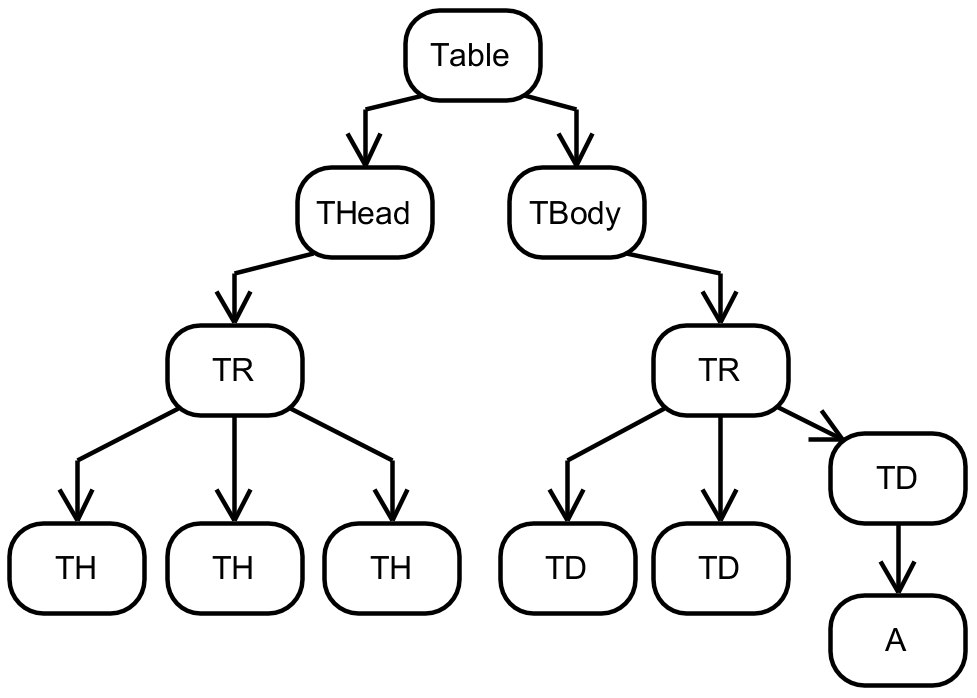
\includegraphics[width=0.5\textwidth]{domTree.png}
\end{center}

\subsection{HTML-формы}

Если надо что-то отправить обратно на сервер, то есть два варианта --- асинхронный запрос из JavaScript (AJAX-запрос, про них чуть позже), либо стандартными средствами HTML, без JavaScript вовсе --- через HTML-форму. Есть тэг \mintinline{html}{<form>}, дочерними тэгами которого должен быть набор тэгов \mintinline{html}{<input>}, один из которых должен иметь type submit:

\begin{minted}{html}
<form method="post">
    First name:<br>
    <input type="text" name="firstName"><br>
    Last name:<br>
    <input type="text" name="lastName"><br><br>
    <input type="radio" name="gender" value="male" checked>Male<br>
    <input type="radio" name="gender" value="female">Female<br>
    <input type="submit" value="Submit">
</form>
\end{minted}

\mintinline{html}{<input>} --- это то, куда пользователь может вводить данные, он может быть разных типов, например, просто строка, кнопка-переключатель, кнопка-флажок и т.д. Когда пользователь жмёт на \mintinline{html}{<input>} типа submit (который выглядит ка обычная кнопка), данные из полей input, введённые пользователем, (или соответствующие им значения атрибута value) сериализуются и отправляются на сервер в виде, как правило, POST-запроса (хотя можно указать желаемый HTTP-метод как атрибут у формы). Сервер может десериализовать присланные данные и что-то с ними сделать (например, сохранить в базу данных), и в конечном итоге он должен в ответ отправить новую HTML-страницу, которую снова отрендерит браузер. Поэтому формы --- это быстрый и простой, но непопулярный нынче метод отправки пользовательского ввода, потому как требует перезагрузки всей страницы. В современном мире это практикуется, и часто даже уместно, когда грузить новую страницу надо и так: например, после авторизации пользователя. Однако всё чаще общение с сервером происходит незаметно для пользователя и без всяких перезагрузок страницы, асинхронными запросами из JavaScript.

\subsection{CSS}

Cascading Style Sheet --- это правильный способ задать внешний вид HTML-документа. CSS --- это, как правило, отдельный файл, на отдельном языке, где описывается, к каким тэгам надо применить какие атрибуты. Cascading оин неспроста, CSS-ок может быть много и они применяются последовательно, возможно, переопределяя друг друга, так что может быть стиль приложения в целом, который переопределяется стилем всех кнопок, который переопределяется стилем конкретной кнопки. При этом атрибуты просто сваливаются в одну кучу (возможно, переопределяя друг друга) и добавляются к соответствующим тэгам, после чего то, что получилось, уже рендерит браузер. Вот так выглядит HTML-документ со <<встроенным>> CSS-ом\footnote{Тут и ниже примеры из \url{https://www.w3schools.com} (дата обращения: 18.11.2021), незаменимого образовательно-справочного ресурса по всему, что свазано с веб-разработкой.} (не делайте так):

\begin{minted}{html}
<!DOCTYPE html>
<html>
    <head>
        <style>
            body {background-color: powderblue;}
            h1   {color: blue;}
            p    {color: red;}
        </style>
    </head>
    <body>
        <h1>This is a heading</h1>
        <p>This is a paragraph.</p>
    </body>
</html>
\end{minted}

А вот тот же HTML-документ, где CSS вынесен в отдельный файл (делайте так):

\begin{minted}{html}
<!DOCTYPE html>
<html>
    <head>
        <link rel="stylesheet" href="styles.css">
    </head>
    <body>
        <h1>This is a heading</h1>
        <p>This is a paragraph.</p>
    </body>
</html>
\end{minted}

В styles.css --- то самое, что было в тэге style выше.

Что происходит в этом примере:

\begin{itemize}
    \item тэгу body выставляется атрибут background-color, равный powderblue;
    \item всем тэгам h1 выставляется атрибут color, равный blue;
    \item всем тэгам p выставляется атрибут color, равный red.
\end{itemize}

Получается очень психоделично свёрстанная страница, так тоже не делайте.

Более тонко настраивать вид тэгов можно с помощью \emph{CSS-селекторов}, которые позволяют фильтровать тэги по типу (это мы как раз только что видели), классу и id. Например:

\begin{minted}{html}
<p id="p01">I am different</p>
<p class="error">Error message</p>
\end{minted}

И соответствующий CSS:

\begin{minted}{css}
#p01 {
    color: blue;
}

p.error {
    color: red;
}
\end{minted}

Несколько селекторов, если они записаны подряд без разделителей, означают <<и>>. Разделитель-пробел означает <<найди сына>>, например, <<div p>> означает выбрать все элементы p внутри всех элементов типа div (при этом сам div такой селектор не выбирает), разделитель-запатая означает <<или>>, например, <<div,p>> означает <<все тэги div и все тэги p>>. Можно делать выборку по атрибутам, селекторами вида <<[attribute]>> и <<[attribute=value]>>. И ещё много чего можно, это странный, но вполне развитый язык запросов к иерархическим данным. Подробности, как обычно, на сайте W3 Schools: \url{https://www.w3schools.com/cssref/css_selectors.asp}.

\subsection{JavaScript}

Наконец, небольшая ликвидация безграмотности по JavaScript. Поскольку рассказывать про синтаксис и модель исполнения JavaScript нет ни времени, ни нужды, ограничимся парой примеров. Вот что-то в духе "Hello, world":

\begin{minted}{html}
<!DOCTYPE html>
<html>
    <body>

    <h1>My First JavaScript</h1>

    <button type="button"
        onclick="document.getElementById('demo').innerHTML = Date()">
        Click me to display Date and Time.
    </button>

    <p id="demo"></p>

    </body>
</html> 
\end{minted}

Тут мы в качестве значения атрибута onclick у button передаём код на JavaScript, который браузер будет исполнять, как нетрудно догадаться, каждый раз, когда пользователь нажимает на кнопку. В нём мы у глобальной переменной document, представляющей тот самый DOM, о котором шла речь выше, вызываем метод getElementById, который возвращает нам элемент по id-шнику, который мы специально для этого навесили на тэг p. Кстати, хорошая практика --- иметь id у всех тэгов, даже если они не используются в скриптах. Это существенно облегчит дальнейшую разработку и, главное, автоматизацию тестирования. У найденного элемента мы меняем внутреннее содержимое (изначально пустое) на результат работы конструктора Date(), который вернёт нам объект типа... нет, который вернёт нам что-то, у чего есть метод toString(), который вернёт нам строку с текущей датой и временем. В JavaScript нет типов в привычном понимании.

Таким же образом можно манипулировать и атрибутами тэгов:

\begin{minted}{html}
<!DOCTYPE html>
<html>
    <head>
        <script>
            function doSomething() {
                document.getElementById("demo").style.fontSize = "25px";
                document.getElementById("demo").style.color = "red";
                document.getElementById("demo").style.backgroundColor = "yellow";
            }
        </script>
    </head>
    <body>
        <button type="button" id="demo" onclick="doSomething()">Click me!</button>
    </body>
</html>
\end{minted}

Тут заодно показано, что в JavaScript есть функции (но они там довольно странные, больше похожие на лямбда-функции в C\#, чем на функции в C, например). И что в HTML есть тэг \mintinline{html}{<script>}, куда можно писать код, который исполнится при загрузке документа (тут при загрузке ничего не произойдёт, потому что мы просто объявили функцию, но не сказали её вызвать). Дальше мы функцию вызываем при вызове обработчика, и всё работает, как в предыдущем примере. Так, конечно, тоже делать не надо, содержательные скрипты, как и CSS-ки, выносят в отдельные файлы .js и ссылаются на них из заголовка страницы (причём, если это библиотека, .js-файл может лежать даже не на вашем сайте, а в CDN\footnote{Content Delivery Network}, обслуживающем эту библиотеку).

Самое интересное, однако, это исполнение асинхронных запросов к серверу. Обратите внимание, запрос по умолчанию можно отправлять только к тому серверу, откуда пришла HTML-страница, и придётся постараться, чтобы переубедить в этом браузер --- так делается из соображений безопасности, в частности, для предотвращения атак Cross Site Scripting (XSS). Для этого есть несколько хороших библиотек (например, axios), но в любом браузере будет без всяких библиотек работать класс XMLHttpRequest (не совсем класс в привычном понимании, но то, что в JavaScript считается классом), что-то вроде HttpClient в .NET. Концептуально всё работает вот так\footnote{картинка, опять же, с \url{https://www.w3schools.com}. Точнее, с \url{https://www.w3schools.com/xml/ajax_intro.asp} (там же можно почитать немного более подробно по теме).}:

\begin{center}
    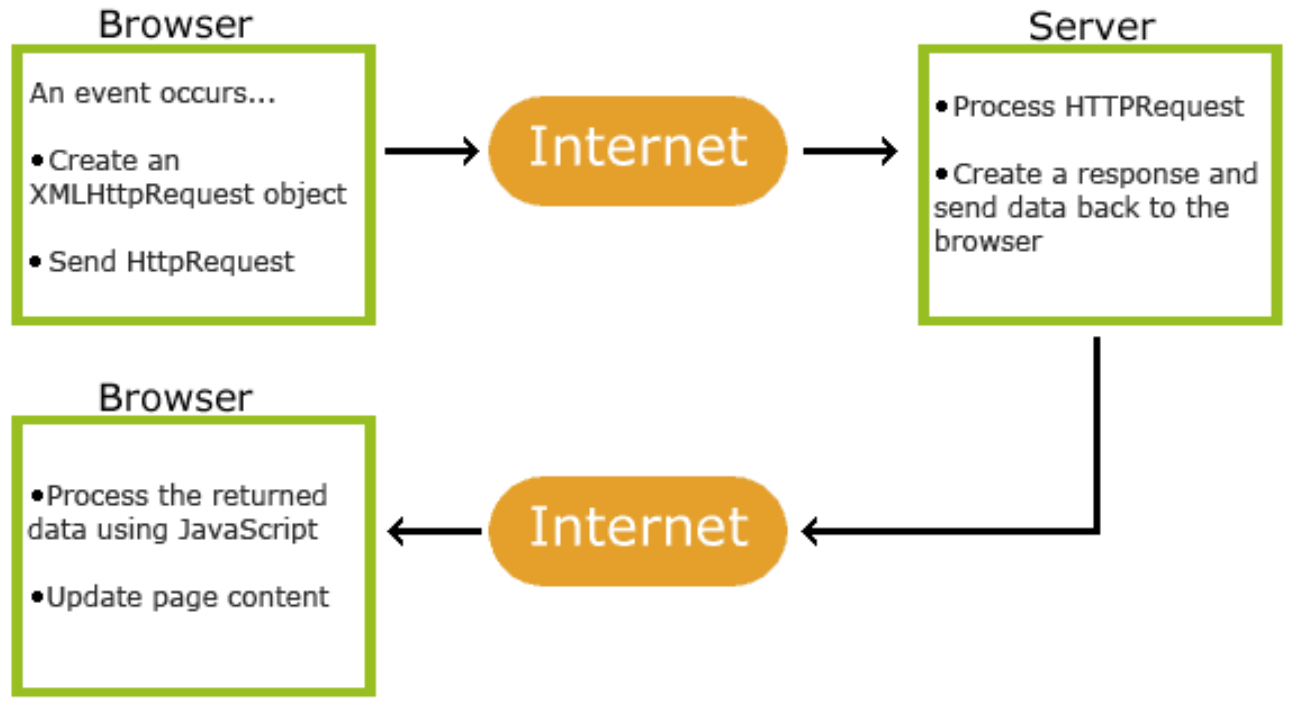
\includegraphics[width=0.7\textwidth]{ajax.png}
\end{center}

Код клиента в браузере, реагируя на какое-то событие (например клик по кнопке), создаёт объект XMLHttpRequest и подписывает коллбэк, который вызовется браузером, когда с сервера придёт ответ. Сам запрос --- это обычный HTTP-запрос, можно указать HTTP-метод, URL (относительно того места, откуда получена страница), и должен быть запрос асинхронным или нет (конечно да). Сервер получает запрос, формирует ответ и отправляет обратно --- как правило, в виде JSON-документа, потому что в JavaScript его даже десериализовывать не нужно, это сразу валидный объект. Браузер принимает ответ от сервера и исполняет коллбэк, который и обновляет содержимое (обычно, хотя может этого не делать). Вот пример:

\begin{minted}{html}
<!DOCTYPE html>
<html>
    <body>
        <div id="demo">
            <h2>The XMLHttpRequest Object</h2>
            <button type="button" onclick="loadDoc()">Change Content</button>
        </div>
        <script>
            function loadDoc() {
            var xhttp = new XMLHttpRequest();
                xhttp.onreadystatechange = function() {
                    if (this.readyState == 4 && this.status == 200) {
                        document.getElementById("demo").innerHTML = this.responseText;
                    }
                };
                xhttp.open("GET", "ajax_info.txt", true);
                xhttp.send();
            }
        </script>
    </body>
</html>
\end{minted}

Тут мы просто делаем на сервер GET-запрос для получения .txt-файла, после чего выставляем его содержимое (просто как текст) вместо кнопки, которая, собственно, и позволила его получить. Тут даже никакой содержательной логики на сервере писать не надо, любой веб-сервер (IIS, Apache) с обработкой такого запроса сам справится.

В какой-то момент (в стандарте ECMA 2017) в JavaScript добавили async/await, уже знакомые по C\# ключевые слова с очень похожей семантикой, так что коллбэки писать стало как-то не очень. Поэтому появился и более современный программный интерфейс для асинхронных запросов, опять-таки, встроенный в браузеры --- Fetch API. Он работает почти везде, кроме, конечно, Internet Explorer, а поскольку есть люди, которые им всё ещё пользуются, то к Fetch API всё ещё есть некое недоверие в сообществе. Зато это гораздо удобнее, гибче и мощнее XMLHttpRequest. Вот небольшой пример\footnote{На сей раз с developer.mozilla.org: \url{https://developer.mozilla.org/en-US/docs/Web/API/Fetch_API/Using_Fetch} (дата обращения: 18.11.2021).}:

\begin{minted}{javascript}
const data = { username: 'example' };

fetch('https://example.com/profile', {
  method: 'POST', // or 'PUT'
  headers: {
    'Content-Type': 'application/json',
  },
  body: JSON.stringify(data),
})
.then(response => response.json())
.then(data => {
  console.log('Success:', data);
})
.catch((error) => {
  console.error('Error:', error);
});
\end{minted}

Через Fetch API можно в принципе делать любые HTTP-запросы, даже файлы загружать (см. \url{https://developer.mozilla.org/en-US/docs/Web/API/Fetch_API/Using_Fetch} для примера).

\subsection{Промежуточное заключение}

Это необходимый минимум, чтобы писать хоть какие-то приложения с фронтендом, но на самом деле это отдельный большой мир, со своими языками, компиляторами/транспиляторами, системами сборки, огромным количеством библиотек, хороших и плохих практик, технических ограничений и т.д. Некоторая очень маленькая часть таких вещей будет рассмотрена в следующей лекции, но надо понимать, что это только вершина айсберга.

Кстати, всё, что мы делали до этого, не требует ничего, кроме браузера и любого текстового редактора. Строго говоря, даже сервера никакого не надо (если не хотите AJAX-запросы попробовать), браузер вполне может отрендерить просто файл .html и даже исполнять оттуда скрипты как ни в чём не бывало. Поэтому есть класс приложений, которые не имеют серверной части вообще и по сути представляют собой размещённые просто где-то .html-файлы со скриптами. Если задача это позволяет, так и надо делать, потому что их очень легко хостить --- <<статическое>> приложение (которое может быть очень даже динамическим, но не требует серверного бэкенда) можно разместить бесплатно, например, на GitHub Pages. Приложения, которым серверная часть хоть в каком-то виде нужна, требуют уже некоторого интеллекта для деплоя --- бесплатные хостинги для них существуют, но предоставляют смехотворное количество вычислительных ресурсов, да и выкладывание таких приложений гораздо более хлопотно.

\section{Бэкенд}

Теперь о том, что происходит на сервере. До того, как запрос попадает на обработку вашему коду, он обрабатывается сетевым стеком операционной системы, который вызывает веб-сервер, который \emph{хостит} ваше веб-приложение. Тут возможны две опции: веб-сервер запущен внутри процесса самого веб-приложения

\end{document}
